\section{What is improvising}

When you want to improvise on the guitar. It's not just playing any chord or note. Instead, it's playing any chord or note within a scale (or outside the scale to be creative).

Most often there will be a certain chord progression played by any instrument in a certain key. Then you can use a scale to improvise a nice melody over it.

\section{The pentatonic scale}

In the last section when we talked about the diminished cord, it was hinted that the pentatonic scale allows you to avoid the restlessness of the tritone interval. But why?

While playing the major and minor scales you may have noticed that half step interval can give some kind of suspension. For example, when you play the 7th note in the major scale, it is only half a step to the root note. Depending on the context, if you play the 7th note, your ear expects the root note to follow.

The pentatonic scale means to have 5 (penta) notes in the scale. Meaning that in general, any 5 notes can form a pentatonic scale. But the pentatonic scale that we know and use is known as the major pentatonic scale. This is the major diatonic scale without the 4th and the 7th note. This removes any semitone tone intervals, and it removes the tritone interval.

\infobox{Note that the word 'removed' was used. This doesn't really does justice to the pentatonic scale. Most likely the pentatonic scale pre-dates the major (diatonic) scale. For example, in 2008 a flute was found that was 30-40 thousand years old and which was tuned to the pentatonic scale. Additionally, Pythagoras studied how the pentatonic scale tones occurred naturally in nature. \cite{PentatonicFlute}}

What the pentatonic scale gives us with this is a \textbf{safer} scale to improvise with. By removing these two notes, we remove the chance that a note that we use while improvising would form a tritone with note that is played in the chord progression for example.

Again, no one is stopping you from going outside the pentatonic scale and be creative. But especially in the beginning, the pentatonic scale is a safe scale for improvising.

\newpage

We will relate the major pentatonic scale to the major (diatonic) scale. You'll see this most often on the internet, and just fits better into the modern western way of thinking about music.

\autoref{tab:guitar_major_pentatic_scale} shows the major pentatonic scale. Here \textbf{W+} means 3 semitones (a whole step (W) + a half step (H)). Note that the indexes are still 1-7 and not 1-5. This is to more easily connect it with the diatonic scales that we've learned in previous chapters.

\begin{table}[h]
	\centering
	\begin{tabular}{*{12}{c}}
		& \multicolumn{2}{P{4mm}}{\large{W}} & \multicolumn{2}{P{4mm}}{\large{W}} & \multicolumn{2}{P{4mm}}{\large{W+}} & \multicolumn{2}{P{4mm}}{\large{W}} & \multicolumn{2}{P{4mm}}{\large{W+}} & \\
		\multicolumn{2}{P{4mm}}{1} & \multicolumn{2}{P{4mm}}{2} & \multicolumn{2}{P{4mm}}{3} & \multicolumn{2}{P{4mm}}{5} & \multicolumn{2}{P{4mm}}{6} & \multicolumn{2}{P{4mm}}{8}
	\end{tabular}
	\caption{Major pentatonic scale intervals}
	\label{tab:guitar_major_pentatic_scale}
\end{table}

For the minor pentatonic scale we remove the 2nd and 6th notes for the same reasons. This results in the following intervals.

\begin{table}[h]
	\centering
	\begin{tabular}{*{12}{c}}
		& \multicolumn{2}{P{4mm}}{\large{W+}} & \multicolumn{2}{P{4mm}}{\large{W}} & \multicolumn{2}{P{4mm}}{\large{W}} & \multicolumn{2}{P{4mm}}{\large{W+}} & \multicolumn{2}{P{4mm}}{\large{W}} & \\
		\multicolumn{2}{P{4mm}}{1} & \multicolumn{2}{P{4mm}}{3} & \multicolumn{2}{P{4mm}}{4} & \multicolumn{2}{P{4mm}}{5} & \multicolumn{2}{P{4mm}}{7} & \multicolumn{2}{P{4mm}}{8}
	\end{tabular}
	\caption{Minor pentatonic scale intervals}
	\label{tab:guitar_minor_pentatic_scale}
\end{table}


That's all nice and well, but how to use this. \autoref{fig:guitar_major_minor_pentatonic_shapes} shows the shape of both the major and minor pentatonic shapes. These are basically the same shapes as the diatonic shapes that you learned earlier, but with some notes removed (4 and 7 for major, 2 and 6 for minor).

\begin{figure}[h]
	\begin{subfigure}[b]{0.45\textwidth}
		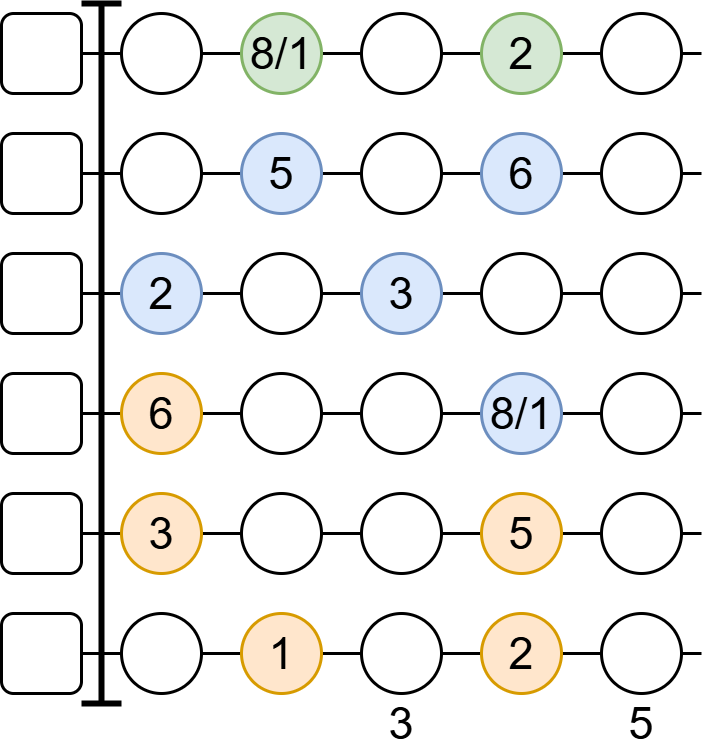
\includegraphics[width=\textwidth]{../../Images/guitar_major_pentatonic_standard.png}
		\caption{Major pentatonic shape}
		\label{fig:guitar_major_pentatonic_shape}
	\end{subfigure}
	\hfill
	\begin{subfigure}[b]{0.45\textwidth}
		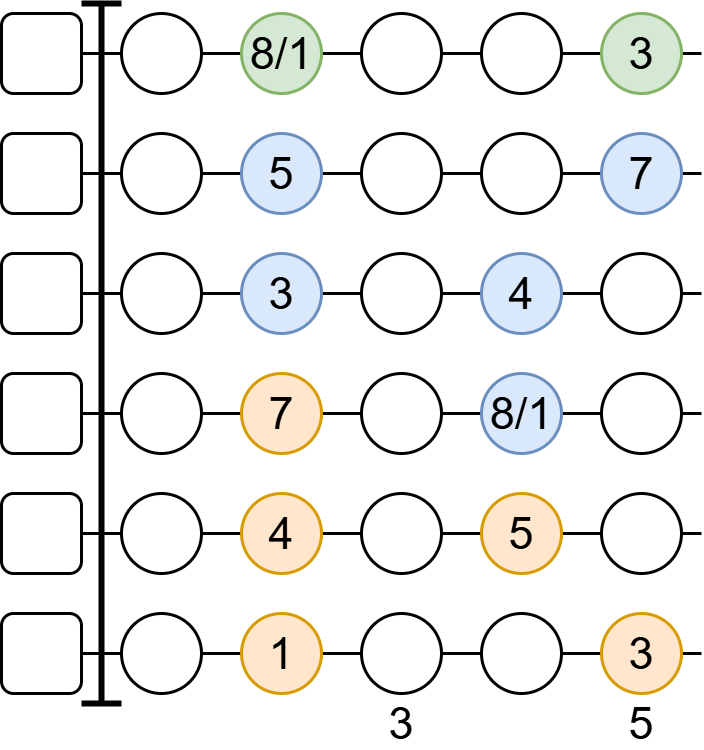
\includegraphics[width=\textwidth]{../../Images/guitar_minor_pentatonic_standard.png}
		\caption{Minor pentatonic shape}
		\label{fig:guitar_minor_pentatonic_shape}
	\end{subfigure}
	\caption{}
	\label{fig:guitar_major_minor_pentatonic_shapes}
\end{figure}

\subsection{Your turn}

Find a song that you like, find the key, and use the pentatonic scale to improvise over the song. The key can often be found on the internet as well.

Note that some songs may change key during the song. This will result in the pentatonic scale to sound a bit off during those parts. When that happens, you can find the key that was switched to and continue in the pentatonic scale in that key.

Another thing you can try is to search for backing tracks in a certain key on the internet.

\newpage

\section{Making it sound more interesting}

\subsection{Legato \& Hammer-On, Pull-Off}
TODO

\subsection{Bending \& Vibrato}
TODO
